% mainfile: ../../../main.tex
\chapter{Vibration spectroscopy}\label{ch:app:setup:vibrations}
\section{Knife-edge measurement}\label{sec:app:setup:vibrations:knife_edge}
\begin{marginfigure}
    \centering
    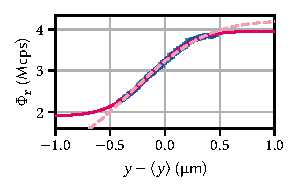
\includegraphics{img/pdf/setup/knife_edge_erf}
    \caption{}
    \label{fig:app:setup:vibrations:knife_edge}
\end{marginfigure}

In \cref{sec:setup:vibrations:optic}, I used a knife-edge measurement to calibrate the readout of the sample position using the count rate of laser radiation reflected off a lateral reflectance gradient.
The gradient was determined by the convolution of the finite spatial extent of the laser spot and a step in reflectance from a \ch{Au} gate with approximately perfect reflectance and the bare \ch{GaAs} surface.
The same measurement can also be used to extract the reflectance $\reflectance_{0}$ of the bare \ch{GaAs} surface as well as the spot size radius $w_0$ of a Gaussian beam by fitting the theoretical dependence of the reflected count rate on the lateral position, \cref{eq:setup:knife_edge}.

From the refractive index of \ch{GaAs}, we would expect
\begin{equation}
    \reflectance_0 = \abs{\frac{n-1}{n+1}}^2 \approx \qty{32}{\percent}
\end{equation}
at zero temperature~\cite{Talghader1995}.
\Cref{fig:app:setup:vibrations:knife_edge} shows the same data as \cref{fig:setup:vibrations:calibration:pos_vs_cps} together with fits to \cref{eq:setup:knife_edge} in magenta.
The dashed line is a fit with $\reflectance_0$ fixed, whereas the solid line is a fit including $\reflectance_0$ as a free parameter.
Clearly, the latter matches the data better, resulting in
\begin{align}
    \reflectance_0 &= \qty{65.1+-1.4}{\percent} \\
    w_0 &= \qty{0.624+-0.028}{\micro\meter}.
\end{align}
The discrepancy in reflectance might be explained by multilayer and thin-film effects given that the sample is only \qty{220}{\nano\meter} thick and warrants closer investigation.
More likely, the assumption that the \ch{Au} optical gate is perfectly reflecting is to be challenged as its thickness corresponds to only a fifth of the wavelength.
In \cref{part:exp}, I carry out \gls{tmm} simulations to this end.
% TODO: Adapt conditioned on TMM simulation results.
The Gaussian beam waist radius $w_0$ resulting from the fit is in quite good agreement with the results obtained in \cref{subsec:setup:optics:coupling:imaging}, where I obtained the value \qty{0.60}{\micro\meter} and \qty{0.84}{\micro\meter} for the $y$- and $z$-direction, respectively (see \cref{tab:setup:optics:coupling:imaging}, but note the different coordinate systems).

\section{Additional vibration spectroscopy data}\label{sec:app:setup:vibrations:data}
% TODO: this
